\documentclass{beamer}

\usepackage[super]{nth}


\title{HVAC Waste Detection - Project Presentation}
\author{Daniele Polidori}
\institute{\textit{Course of Internet of things}\\
\textit{University of Bologna}}
\date{Academic year 2023-24}

\setbeamertemplate{navigation symbols}{\tiny\insertframenumber}     % Inserisce il numero di pagina al posto dei simboli di navigazione
\setbeamercolor{navigation symbols}{fg=black}   % Colora di nero i simboli di navigazione


\begin{document}


{
\setbeamertemplate{footline}{}      % Elimina il footline in questa slide
\setbeamertemplate{navigation symbols}{}    % Lascia uno spazio vuoto al posto dei simboli di navigazione
\begin{frame}
 \titlepage     % Beamer's \maketitle
\end{frame}
}
%\addtocounter{framenumber}{-1}     % Non considera questa slide nel conteggio delle pagine


\begin{frame}{Introduction}

	I realized an IoT system that monitors the temperature of an house, to prevent useless HVAC consumption, detecting it by rapid temperature changes.
	
	\vfill

	\begin{block}

		\begin{columns}[onlytextwidth,T]
		
			\column{\dimexpr\linewidth-50mm-5mm}

			Composed by an \textbf{ESP-WROOM-32} board\\linked to:
			\begin{itemize}
				\item 1 \textbf{indoor DHT22} sensor,
				\item 1 \textbf{outdoor DHT22} sensor,
				\item 1 \textbf{LED}.
			\end{itemize}

			\column{50mm}
			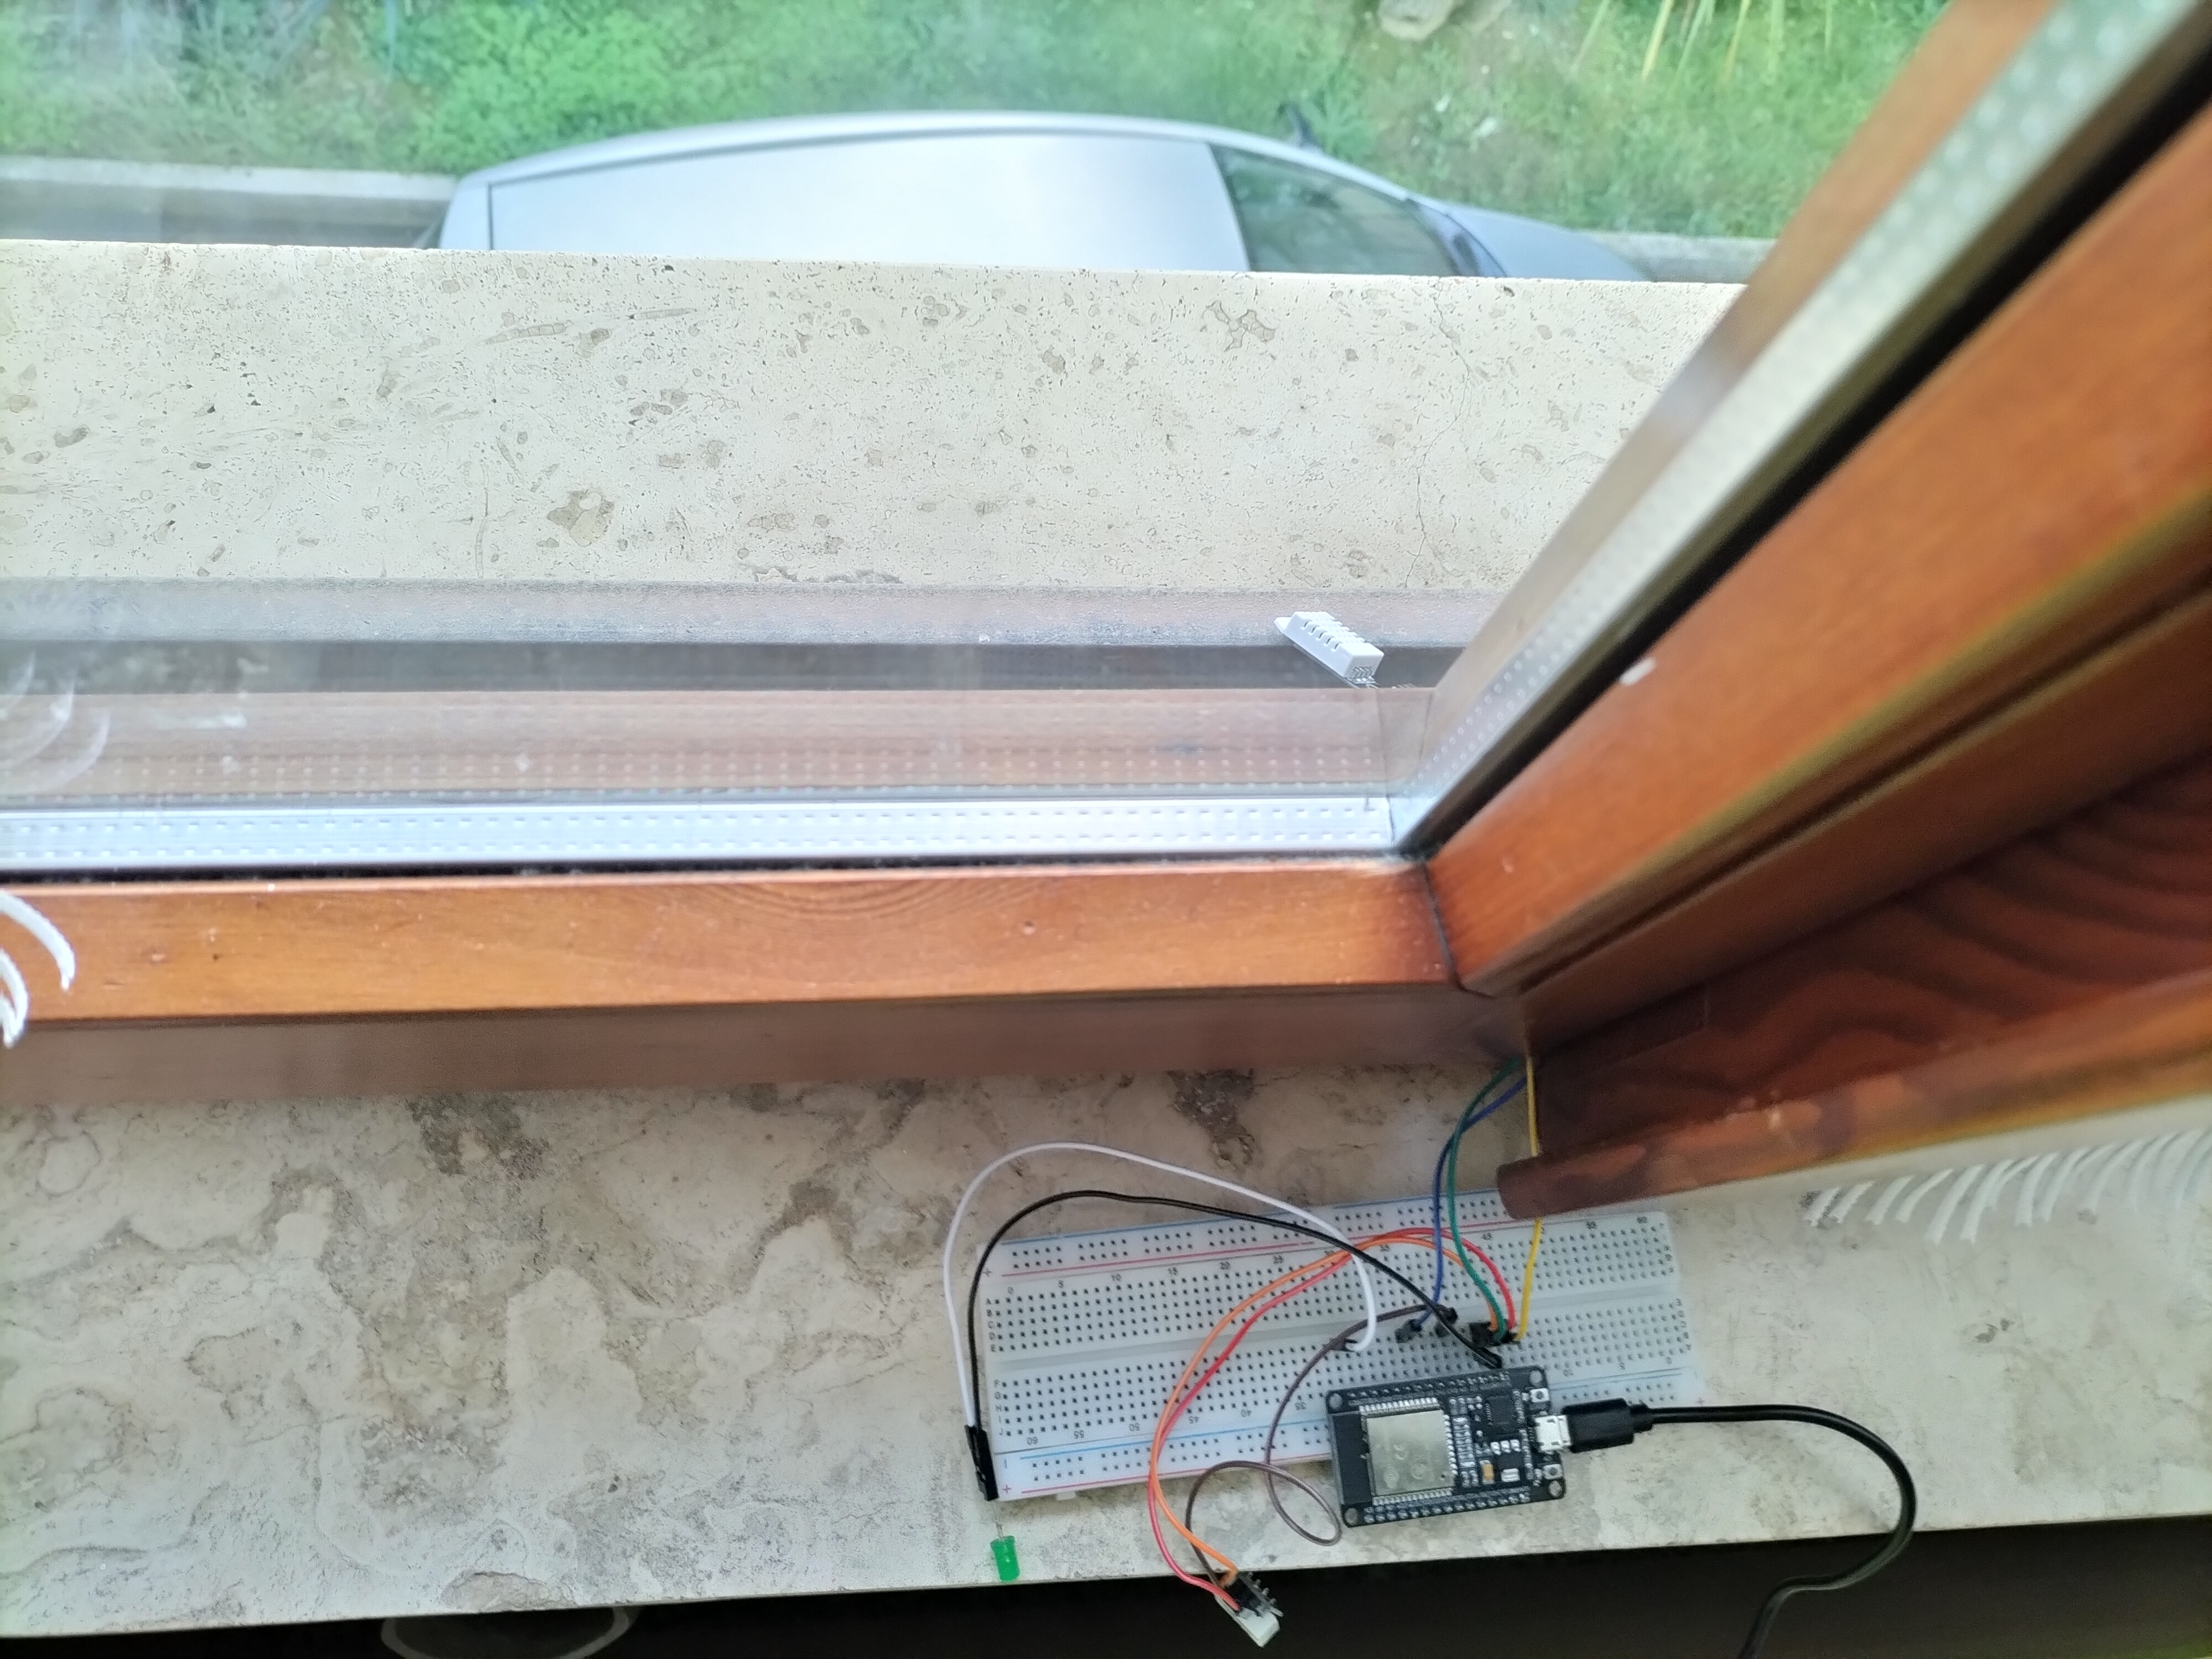
\includegraphics[scale=0.035]{figures/figure_esp.jpg}

		\end{columns}
	\end{block}
\end{frame}


\begin{frame}{Data acquisition - ESP32}

	\begin{description}[\texttt{PubSubClient}]		% Indico la lunghezza della label piu' lunga, cosi' che siano tutte allineate a dx
		\item[\texttt{Thing.CoAP}]: To act as a CoAP server.
		\item[\texttt{PubSubClient}]: To act as a MQTT subscriber.
	\end{description}

	\vfill

	Through the CoAP protocol, the ESP32 is able to send the latest collected indoor and outdoor temperature value, when asked.

	\vfill

	Through the MQTT protocol, the board can receive some commands:
	\begin{itemize}
		\item to start or stop the sensors reading,
		\item to change the interval between consecutive sensors readings,
		\item to turn on or off the LED.
	\end{itemize}
	My laptop acts as a MQTT broker, through Mosquitto.

\end{frame}


\begin{frame}{Data proxy - \nth{1} Python script}

	\begin{description}[\texttt{influxdb-client}]		% Indico la lunghezza della label piu' lunga, cosi' che siano tutte allineate a dx
		\item[\texttt{paho-mqtt}]: To act as a MQTT publisher.
		\item[\texttt{aiocoap}]: To act as a CoAP client.
		\item[\texttt{influxdb-client}]: To store data.
	\end{description}

	\vfill

	Initially, through the MQTT protocol, the application gives commands, to the ESP32, to start the sensors reading and to set their sampling rate.
	
	\vfill
	
	Periodically, through the CoAP protocol, the script requests, to the board, the latest collected indoor and outdoor temperature value. It continuously stores these values on a local InfluxDB instance.\\
	
	\vfill
	
	The network latency, between the temperature value request and its reception, is continuously monitored; after a while, the script evaluates the mean latency of this process.

\end{frame}


\begin{frame}{Data analytics - \nth{2} Python script (1/2)}

	\begin{description}[\texttt{influxdb-client}]		% Indico la lunghezza della label piu' lunga, cosi' che siano tutte allineate a dx
		\item[\texttt{influxdb-client}]: To get and store data on the database.
		\item[\texttt{prophet}]: To forecast future temperature values.
		\item[\texttt{paho-mqtt}]: To act as a MQTT publisher.
	\end{description}

	\vfill

	At the beginning, the script gets all past temperature values from the database to make a prediction of some indoor and outdoor future values. As the forecasted temperature times are reached, the application stores the predicted values on the database.
	
	\vfill
	
	Ciclically, the application retrieves some of the latest temperature values from the database and analyses them to check a possible HVAC waste.\\
	When the alarm goes off, the script stores the alarm event on the database and, through the MQTT protocol, gives the command, to the ESP32, to turn on the LED; when the risk has passed, the script gives the command to turn it off.

\end{frame}


\begin{frame}{Data analytics - \nth{2} Python script (2/2)}

	The alarm goes off if:
	\begin{itemize}
		\item the indoor temperature is changing rapidly \eqref{eq_varianza} and
		\item the indoor temperature is approaching the outdoor one \eqref{eq_media}.
	\end{itemize}
	
	\vfill
	
	Mathematically speaking:
	\begin{equation}
	var(i_1, i_2, \dots, i_n) > threshold \label{eq_varianza}
	\end{equation}
	\begin{equation}
	min(i_n, o_n) < mean(i_1, i_2, \dots, i_n) < max(i_n, o_n) \label{eq_media}
	\end{equation}
	where $i$ is the indoor temperature, $o$ is the outdoor temperature and $t_1, t_2, \dots, t_n$ are the $n$ latest temperature values retreived: $t_1$ is the newest and $t_n$ is the farthest.

\end{frame}


\begin{frame}{Data visualization}

	\begin{block}

		\begin{columns}[onlytextwidth,T]
		
			\column{\dimexpr\linewidth-65mm-5mm}

			Local Grafana instance that shows:
			\begin{itemize}
				\item the collected temperature values,
				\item the forecasted ones,
				\item the counting of the alarm events.
			\end{itemize}

			\column{68mm}
			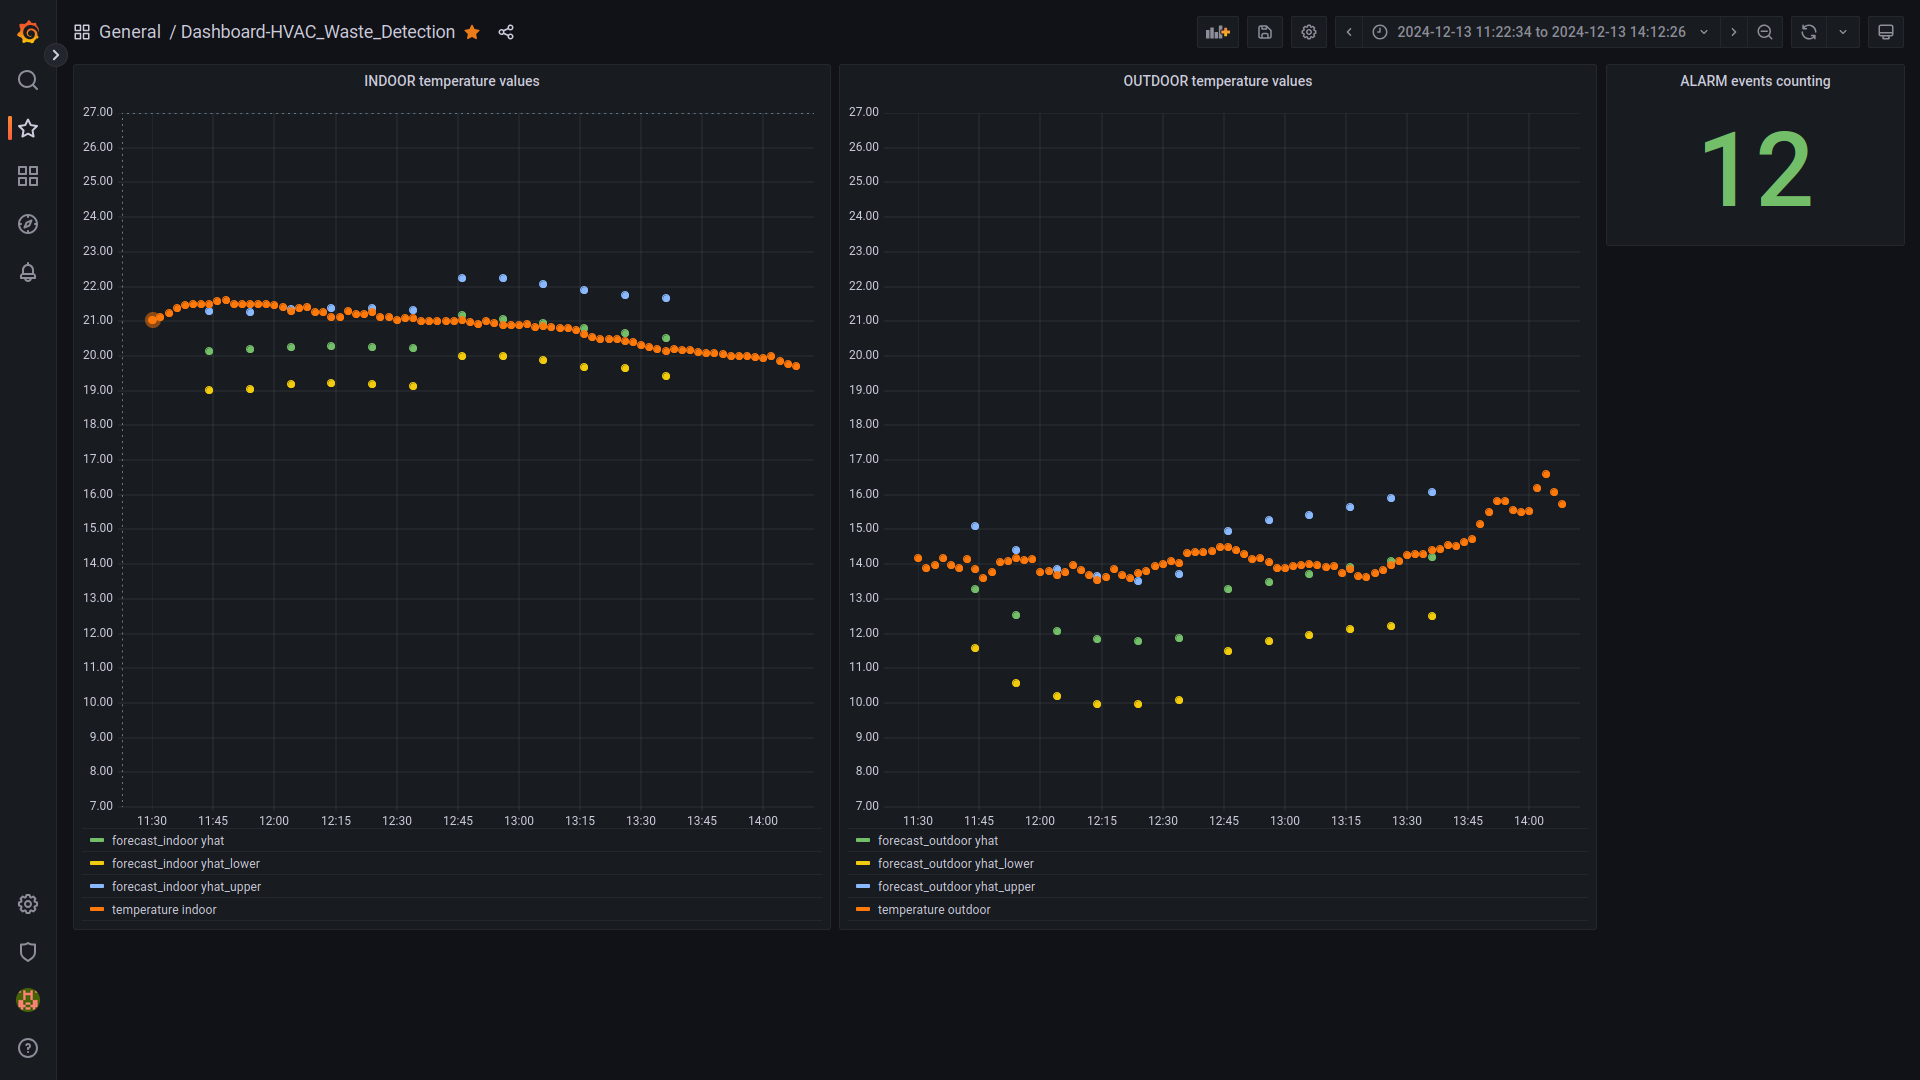
\includegraphics[scale=0.1]{figures/figure_grafana.png}

		\end{columns}
	\end{block}
\end{frame}


\end{document}
